% Provenance (never printed): see sources/outline_sources.md (Year 1: rigid plates on a
% sphere, Euler poles and angular velocities; relative velocities; triple junctions;
% finite rotations; the magnetic-anomaly timescale; satellite geodesy). Curves and maps
% from figdata/bachelor-1/euler_velocities.py, south_atlantic_fit.py and gpts_stripes.py;
% exercise and problem values in the Book 3 scratch calculator calc/ch12.py.
\chapter{球面上的板块运动学}\label{ch:b1:plate-kinematics}

两个卫星定位站每天记录其位置，
已超过四分之一世纪：一站位于冰岛西部的雷克雅未克，
另一站位于挪威西海岸附近的斯塔万格。两站之间的直线
长 \qty{1546}{km}，每年增长 \qty{17.5}{mm}，
接近两厘米。地面上看不出任何迹象，但两站之间
的北大西洋洋底记录了数百万年间同样的张开：大西洋中脊喷出的熔岩
冷却时获得了地磁场的方向，
而地磁场已多次倒转，因此
洋底保留了自身生长的条带状记录。本章
把中学阶段的板块看作球面上的刚性帽，用旋转几何描述
它们的运动，并说明地质
记录与卫星如何测量同一运动。
% ledger: ngl:reyk, ngl:stas (chord lengthening computed in calc/ch12.py)

\begin{recall}
在球面上，\omterm{def:b1:spherical-astronomy:spherical-triangle}{大圆}是过球心的平面与球面的交线，
\omterm{def:b1:spherical-astronomy:spherical-triangle}{小圆}是任一其他平面与球面的交线；余弦定理由两点的\omterm{def:b1:spherical-astronomy:geographic}{纬度}与\omterm{def:b1:spherical-astronomy:geographic}{经度}
给出两点间的角距离，并且
方向的\omterm{def:b1:spherical-astronomy:horizontal}{方位角}自北经东计量
（见\cref{ch:b1:spherical-astronomy}）。绕固定轴转动的刚体具有
角速度（物理）。\omterm{def:b1:layered-earth:lithosphere}{岩石圈}被分成若干板块，它们彼此相对运动，
速率约为每年几厘米；洋底保留着
记录了地磁场倒转的
磁场倒转的磁条带（第 2 册，十一年级）。
\end{recall}

\section{球面上的刚性板块}

一个板块覆盖球面的很大一部分：欧亚板块从
大西洋中部延伸到西伯利亚东部。其运动不能像汽车那样用速度描述，
而必须用旋转来描述。

\begin{definition}[刚性板块]\label{def:b1:plate-kinematics:rigid-plate}
称\omterm{def:b1:layered-earth:lithosphere}{岩石圈}中的一个区域为\emph{刚性板块}\index{刚性板块}，其
内部不发生可测变形，即其中任意两点间的距离
保持不变。两个板块的相对运动由它们的
公共边界承担，该边界是由断层、地震和火山组成的狭窄地带。
\end{definition}

没有任何板块是绝对刚性的：边界是宽数十至数百
千米的地带，内部则缓慢变形。这一假设认为这些
偏离量远小于相对运动；该假设由
本章所有结果的一致性加以检验。

球面上的\omterm{def:b1:plate-kinematics:rigid-plate}{刚性板块}运动时，其上任意两点之间的距离
保持不变，地球中心不动。这种运动
可用一个 $3\times3$ 矩阵 $R$ 描述，它保持长度，
是\emph{正交}矩阵（$R^{\mathsf T}R = I$），并保持空间的
定向，即 $\det R = 1$：位置矢量为 $\vec r$ 的点映为
$R\vec r$。

\begin{theorem}[欧拉旋转定理]\label{thm:b1:plate-kinematics:euler}
球面上\omterm{def:b1:plate-kinematics:rigid-plate}{刚性板块}的每一个位移，都是绕一条
过地心的轴的旋转：存在单位矢量 $\vec n$，使得
$R\vec n = \vec n$，且板块绕 $\vec n$ 转过某一角度。
\end{theorem}

\begin{proof}
只需证明 $1$ 是 $R$ 的本征值，即 $\det(R - I) = 0$。由
$R R^{\mathsf T} = I$，得 $R - I = R(I - R^{\mathsf T})$，于是
\[
  \det(R - I) = \det R\,\det\bigl((I - R)^{\mathsf T}\bigr) = \det(I - R),
\]
利用 $\det R = 1$ 以及矩阵与其转置具有相同的
行列式。对 $3\times3$ 矩阵，
$\det(I - R) = (-1)^3\det(R - I) = -\det(R - I)$。于是 $\det(R - I) =
-\det(R - I)$，即其为零。单位矢量 $\vec n$ 满足 $R\vec n = \vec n$，
因此存在：过球心沿
$\vec n$ 所指方向的直线与球面的两个交点不动。在垂直于 $\vec n$ 的平面内，
$R$ 保持长度与定向：它使该平面转过某一角度，于是
因此也使整个球面绕 $\vec n$ 转动。
\end{proof}

在运动不变的足够短时间间隔内，
旋转以\omterm{def:b1:plate-kinematics:triple-junction}{稳定}的速率进行，一个板块相对于
另一板块的运动是绕固定轴的角速度。

\begin{definition}[欧拉极；欧拉矢量]\label{def:b1:plate-kinematics:euler-pole}
板块 B 相对于板块 A 的运动是绕一条
过地心的轴的旋转。这一对板块的\emph{欧拉极}\index{欧拉极}是
该轴与球面相交的点，选取使
从该极上方看旋转为逆时针；对跖点是
对极。\emph{欧拉矢量}\index{欧拉矢量}
$\vec\omega_{BA}$ 是 B 相对于 A 的角速度：它由
地心指向欧拉极，其长度 $\omega$ 即
转动速率。
\end{definition}

\omterm{def:b1:plate-kinematics:euler-pole}{欧拉矢量}由其极的\omterm{def:b1:spherical-astronomy:geographic}{纬度}、\omterm{def:b1:spherical-astronomy:geographic}{经度}和
转动速率给出，通常以度每百万年计。欧亚板块的运动
相对于北美板块，平均取最近 \qty{3.16}{Ma}
内由两板块之间洋脊上测得的 453 个扩张速率求得，其极位于
北纬 \ang{61.8}，东经 \ang{139.6}，即西伯利亚东部，转动速率为
\qty{0.210}{\degree\per\Ma}。换算为弧度每年：
\[
  \omega = \frac{0.210\times\pi/180}{\num{e6}} = \qty{3.665e-9}{rad.\text{年}^{-1}},
\]
转一整圈需 \qty{1714}{\Ma}。
% ledger: morvel:eu-na, morvel:summary

\section{相对速度}

\begin{theorem}[旋转板块上的速度]\label{thm:b1:plate-kinematics:velocity}
若板块 B 相对于板块 A 以\omterm{def:b1:plate-kinematics:euler-pole}{欧拉矢量} $\vec\omega$ 转动，
则 B 上位置矢量（自地心算起）为 $\vec r$ 的点
相对 A 的速度为：
\[
  \vec v = \vec\omega\times\vec r .
\]
\end{theorem}

\begin{proof}
设 $\Delta$ 为 $\vec\omega$ 与 $\vec r$ 的夹角。当 B 转动时，
该点绕转轴描出一个圆，其半径为 $R\sin\Delta$，其中 $R$ 为
地球半径；以角速率 $\omega$ 转动时，其速率为
$\omega R\sin\Delta$。其速度与该圆相切，因此垂直于转轴
及半径 $\vec r$，又转动为绕 $\vec\omega$ 的逆时针方向，
其指向与 $\vec\omega\times\vec r$ 相同。
矢量 $\vec\omega\times\vec r$ 的方向与指向恰与此相同，
且长度为 $\omega R\sin\Delta$。
\end{proof}

角 $\Delta$ 即\omterm{def:b1:plate-kinematics:euler-pole}{欧拉极}与该点之间的角距离，
其值可由余弦定理利用\omterm{def:b1:spherical-astronomy:geographic}{纬度}与\omterm{def:b1:spherical-astronomy:geographic}{经度}求得。

\begin{proposition}[相对运动的速率与方向]\label{prop:b1:plate-kinematics:speed}
设\omterm{def:b1:plate-kinematics:euler-pole}{欧拉极}位于\omterm{def:b1:spherical-astronomy:geographic}{纬度} $\varphi_p$、\omterm{def:b1:spherical-astronomy:geographic}{经度} $\lambda_p$，
某点位于\omterm{def:b1:spherical-astronomy:geographic}{纬度} $\varphi$、\omterm{def:b1:spherical-astronomy:geographic}{经度} $\lambda$。则
\begin{enumerate}
  \item 自极点到该点的角距离 $\Delta$ 满足
        $\cos\Delta = \sin\varphi_p\sin\varphi + \cos\varphi_p\cos\varphi
        \cos(\lambda - \lambda_p)$；
  \item 相对速度为 $v = \omega R\sin\Delta$：在极点处为零，
        在距极点 \ang{90} 的\omterm{def:b1:spherical-astronomy:spherical-triangle}{大圆}上最大，为 $\omega R$；
  \item 运动方向垂直于连接该点与极点的\omterm{def:b1:spherical-astronomy:spherical-triangle}{大圆}，
        其\omterm{def:b1:spherical-astronomy:horizontal}{方位角}等于从该点望向极点的\omterm{def:b1:spherical-astronomy:horizontal}{方位角}，
        再加 \ang{90}。
\end{enumerate}
\end{proposition}

\begin{proof}
（1）是对由地理北极、
\omterm{def:b1:plate-kinematics:euler-pole}{欧拉极}与该点所构成的\omterm{def:b1:spherical-astronomy:spherical-triangle}{球面三角形}应用余弦定理，其自北极出发的两边分别为
$\ang{90} - \varphi_p$ 与 $\ang{90} - \varphi$，两边夹角为
$\lambda - \lambda_p$。（2）由定理即得。（3）
速度垂直于 $\vec\omega$ 与 $\vec r$，故垂直于二者所在的
平面，即过该点与极点的\omterm{def:b1:spherical-astronomy:spherical-triangle}{大圆}所在平面。在
该点的水平面内，因此它垂直于
极点方向；转动自极点上方看为逆时针，
即质点沿其望见极点的方向的右侧运动，
这使\omterm{def:b1:spherical-astronomy:horizontal}{方位角}增加 \ang{90}。
\end{proof}

\begin{omfigure}
\begin{tikzpicture}[x=2.5cm, y=2.5cm, font=\scriptsize, >=Stealth]
% orthographic view from 20 deg above the "Euler equator": a point at polar angle D,
% longitude p about the pole projects to X = sin D sin p, Y = cos D cos 20 - sin D cos p sin 20;
% it is visible when cos p >= -cot D tan 20 (limits computed by hand: 129.08, 102.13, 90, 77.87)
\fill[omSea!12] (0,0) circle (1);
\draw[thick] (0,0) circle (1);
\foreach \D/\m in {30/129.08, 60/102.13, 90/90, 120/77.87} {
  \draw[blue!45!black, domain=-\m:\m, samples=60, variable=\p]
    plot ({sin(\D)*sin(\p)}, {cos(\D)*cos(20) - sin(\D)*cos(\p)*sin(20)});
  \draw[blue!45!black, densely dashed, domain=\m:360-\m, samples=60, variable=\p]
    plot ({sin(\D)*sin(\p)}, {cos(\D)*cos(20) - sin(\D)*cos(\p)*sin(20)});
}
\draw[densely dashed] (0,0) -- (0,0.9397);
\draw[->, very thick] (0,0.9397) -- (0,1.38) node[above] {$\vec\omega$};
\fill (0,0.9397) circle (0.9pt) node[anchor=south west] {欧拉极};
\fill (0,0) circle (0.7pt);
% velocity arrows at longitude -35 deg about the pole, length 0.5 sin D
\draw[->, very thick, red!75!black] (-0.287,0.6737) -- ++(0.243,-0.058);
\draw[->, very thick, red!75!black] (-0.497,0.2272) -- ++(0.421,-0.101);
\draw[->, very thick, red!75!black] (-0.574,-0.2802) -- ++(0.487,-0.117);
\draw[->, very thick, red!75!black] (-0.497,-0.7124) -- ++(0.421,-0.101);
\draw[->] (0,0) -- (-0.497,0.2272) node[pos=0.55, below] {$\vec r$};
\draw (0,0.22) arc[start angle=90, end angle=155.4, radius=0.22];
\node at (-0.11,0.33) {$\Delta$};
\node[anchor=west] at (0.62,0.81) {$\Delta = \ang{30}$};
\node[anchor=west] at (0.88,0.47) {$\Delta = \ang{60}$};
\node[anchor=west] at (1.02,0.0) {$\Delta = \ang{90}$};
\node[anchor=west] at (0.88,-0.47) {$\Delta = \ang{120}$};
\end{tikzpicture}

\par\smallskip{\small 绕其\omterm{def:b1:plate-kinematics:euler-pole}{欧拉极}转动的板块，自距极点 \ang{90}
的圆上方略高处看去。每一点都沿绕极点的\omterm{def:b1:spherical-astronomy:spherical-triangle}{小圆}运动（被遮挡部分用虚线表示）；
其速率由红色箭头表示，为
$\omega R\sin\Delta$，其中 $\Delta$ 为其与极点的角距离：
在极点处为零，在距极点 \ang{90} 处最大。}
\label{fig:b1:plate-kinematics:euler-pole}
\end{omfigure}

因此，相对运动的速率沿板块边界变化，即使
两板块完全刚性，运动方向也随之转动。
两个推论决定了每一张板块边界图的面貌。

\begin{proposition}[转换断层沿小圆分布]\label{prop:b1:plate-kinematics:transforms}
两板块相互错动而既不张开也不闭合的转换断层，
位于以两板块\omterm{def:b1:plate-kinematics:euler-pole}{欧拉极}为中心的一个\omterm{def:b1:spherical-astronomy:spherical-triangle}{小圆}上。
洋中脊处的扩张方向，以及俯冲带处的汇聚方向，
同样沿这些\omterm{def:b1:spherical-astronomy:spherical-triangle}{小圆}方向。
\end{proposition}

\begin{proof}
在转换断层上，相对速度在各点处都与断层平行。
相对速度处处与绕极点的\omterm{def:b1:spherical-astronomy:spherical-triangle}{小圆}相切
（见\cref{thm:b1:plate-kinematics:velocity}）；若曲线在其每一点处都与
经过该点的\omterm{def:b1:spherical-astronomy:spherical-triangle}{小圆}相切，则它即为这些\omterm{def:b1:spherical-astronomy:spherical-triangle}{小圆}之一。
第二个论断即\cref{prop:b1:plate-kinematics:speed}的第三部分。
\end{proof}

欧亚板块与北美板块之间的大西洋中脊，是一串阶梯状排列的洋脊段，
各段之间由转换断层错开；转换断层的\omterm{def:b1:field-lab-methods-1:trend-plunge}{倾伏向}接近
\omterm{def:b1:plate-kinematics:euler-pole}{欧拉矢量}所预言的\omterm{def:b1:spherical-astronomy:horizontal}{方位角}，而它们的\omterm{def:b1:field-lab-methods-1:trend-plunge}{倾伏向}正是用来
定位\omterm{def:b1:plate-kinematics:euler-pole}{欧拉极}的数据之一。沿同一边界的扩张速率随
离极点的角距离增大：北冰洋的 Gakkel
洋脊靠近极点，速率为 \qtyrange{11}{12}{mm.\text{年}^{-1}}；而
就在亚速尔群岛以北，速率为 \qty{23}{mm.\text{年}^{-1}}，距极点 \ang{78}。下图比较\omterm{def:b1:plate-kinematics:euler-pole}{欧拉矢量}
沿整段边界预言的速率与一个独立板块模型给出的速率。
% ledger: morvel:eu-na

\begin{method}[某点处的速度]\label{met:b1:plate-kinematics:velocity}
\begin{enumerate}
  \item 将\omterm{def:b1:plate-kinematics:euler-pole}{欧拉矢量}的速率换算为每年弧度，并计算
        $\omega R$，单位为 \unit{mm.\text{年}^{-1}}，其中 $R = \qty{6371}{km}$。
  \item 计算从极点到该点的角距离 $\Delta$，
        用余弦定理求得，速率为 $\omega R\sin\Delta$。
  \item 计算从该点看去极点的\omterm{def:b1:spherical-astronomy:horizontal}{方位角} $\beta$，
        $\tan\beta = \sin(\lambda_p - \lambda)\cos\varphi_p /
        \bigl(\cos\varphi\sin\varphi_p - \sin\varphi\cos\varphi_p
        \cos(\lambda_p - \lambda)\bigr)$，象限由分子与
        分母共同确定；运动朝向 $\beta + \ang{90}$。
  \item 检查方向：该运动是第二块板块相对于
        第一块板块的运动，交换两板块则方向相反。
\end{enumerate}
\end{method}

\begin{example}[欧亚板块在冰岛远离北美板块]\label{ex:b1:plate-kinematics:iceland}
取冰岛中部，其坐标为北纬 \ang{64.5}、西经 \ang{18}，并取
上文所给欧亚板块相对北美板块的\omterm{def:b1:plate-kinematics:euler-pole}{欧拉矢量}。于是 $\omega R =
\num{3.665e-9}\times\qty{6.371e9}{mm} = \qty{23.35}{mm.\text{年}^{-1}}$，由下式
\[
  \cos\Delta = \sin\ang{61.8}\sin\ang{64.5}
  + \cos\ang{61.8}\cos\ang{64.5}\cos(\ang{-18} - \ang{139.6}) = 0.60736,
\]
可得 $\Delta = \ang{52.60}$，$v = 23.35\sin\ang{52.60} = \qty{18.55}{mm.\text{年}^{-1}}$。
从冰岛看去，极点位于\omterm{def:b1:spherical-astronomy:horizontal}{方位角} $\beta = \ang{13.1}$ 处，即北偏东一点，
位于北极上空；欧亚板块朝 $\ang{103.1}$ 方向运动，即东南偏东，也就是
向东 \qty{18.07}{mm.\text{年}^{-1}}，向南 \qty{4.20}{mm.\text{年}^{-1}}。
% computed in calc/ch12.py and figdata/bachelor-1/euler_velocities.py
\end{example}

\begin{omfigure}
\begin{tikzpicture}
\begin{axis}[omrecord, width=0.84\linewidth, height=6.4cm, xmin=0, xmax=90, ymin=0, ymax=26,
  xtick={0,15,...,90}, xlabel={距欧拉极的角距离，$\Delta$（度）},
  ylabel={扩张速率（\unit{mm.\text{年}^{-1}}）},
  legend style={font=\scriptsize, at={(0.99,0.03)}, anchor=south east, draw=none, fill=white, fill opacity=0.85, text opacity=1},
  legend cell align=left]
% computed in figdata/bachelor-1/euler_velocities.py
\addplot[only marks, mark=*, mark size=0.9pt, black!55] table[x=delta, y=pb2002] {figdata/out/bachelor-1-euler_velocities-mar.dat};
\addlegendentry{板块边界模型 PB2002，每个边界步}
\addplot[only marks, mark=x, mark size=1.1pt, blue!60!black] table[x=delta, y=gps] {figdata/out/bachelor-1-euler_velocities-mar.dat};
\addlegendentry{卫星定位得到的欧拉矢量}
\addplot[very thick, red!75!black] table[x=delta, y=v] {figdata/out/bachelor-1-euler_velocities-curve.dat};
\addlegendentry{$\omega R\sin\Delta$，地质欧拉矢量}
\node[font=\scriptsize, anchor=south east] at (axis cs:52.6,19.6) {冰岛};
\draw[black!70] (axis cs:52.6,18.55) circle (2.5pt);
\node[font=\scriptsize, anchor=south] at (axis cs:78.4,23.6) {亚速尔};
\draw[black!70] (axis cs:78.4,22.87) circle (2.5pt);
\node[font=\scriptsize, anchor=south] (gk) at (axis cs:9,12) {Gakkel 洋脊};
\draw[black!70, -{Stealth[length=3pt]}] (gk.south) -- (axis cs:16.5,7.2);
\end{axis}
\end{tikzpicture}

\par\smallskip{\small 欧亚板块与北美板块之间的扩张速率，从
北冰洋至亚速尔群岛一段，随距\omterm{def:b1:plate-kinematics:euler-pole}{欧拉
极}的角距离而变化。红色为地质\omterm{def:b1:plate-kinematics:euler-pole}{欧拉矢量}（极点北纬 \ang{61.8}、东经 \ang{139.6}，
\qty{0.210}{\degree\per\Ma}），所有速率均落在同一条正弦曲线上。灰色为
独立板块边界模型在各边界步上的速率；
它们与该曲线平均相差 \qty{1}{\percent}。蓝色为
在相同各步处，由两板块内部的卫星定位算得的\omterm{def:b1:plate-kinematics:euler-pole}{欧拉矢量}所预言的速率，
（极点北纬 \ang{74.2}、东经 \ang{134.1}，
\qty{0.237}{\degree\per\Ma}）：极点位于别处，其速率不落在
红色曲线上。它们在亚速尔至冰岛之间，与地质速率相差不到十分之一，
而在北极地区明显偏低，那里速率很小，且
强烈依赖于极点的确切位置。}
\label{fig:b1:plate-kinematics:mar-rates}
\end{omfigure}
% ledger: morvel:eu-na, morvel:gps-eu-na, data:pb2002 (mean difference 0.96 per cent, euler_velocities.py)

\section{运动的合成；三联点}

相对速度与力学中的速度一样可以相加：若 B 相对
A 运动，C 相对 B 运动，则 C 相对 A 的运动为
两速度之和。

\begin{proposition}[欧拉矢量可加]\label{prop:b1:plate-kinematics:addition}
设三块板块 A、B、C，
\[
  \vec\omega_{CA} = \vec\omega_{CB} + \vec\omega_{BA}, \qquad
  \vec\omega_{AB} = -\vec\omega_{BA}.
\]
\end{proposition}

\begin{proof}
对每一点 $\vec r$，$\vec v_{CA} = \vec v_{CB} + \vec v_{BA}$，即
$\vec\omega_{CA}\times\vec r = \vec\omega_{CB}\times\vec r +
\vec\omega_{BA}\times\vec r = (\vec\omega_{CB} + \vec\omega_{BA})\times\vec r$
由叉积的线性性质。若矢量 $\vec u$ 满足
$\vec u\times\vec r = \vec 0$ 对每个 $\vec r$ 成立，则该矢量为零，故两\omterm{def:b1:plate-kinematics:euler-pole}{欧拉矢量}
相等。交换 A 与 B，所有速度均反向。
\end{proof}

要将\omterm{def:b1:plate-kinematics:euler-pole}{欧拉矢量}相加，先将各矢量写为直角坐标分量，即 $\omega(\cos\varphi_p
\cos\lambda_p, \cos\varphi_p\sin\lambda_p, \sin\varphi_p)$，各分量相加，
再换算回极点与速率。极点不能相加，\omterm{def:b1:plate-kinematics:euler-pole}{欧拉矢量}
可以相加。这一关系是很有力的约束。努比亚板块
（非洲）相对欧亚板块的运动很慢，地质记录给出的
直接测量很少：在亚速尔与直布罗陀之间，仅有的测量是
一条转换断层（Gloria 断层）的\omterm{def:b1:spherical-astronomy:horizontal}{方位角}。它转而由
横跨大西洋、测量良好的两组扩张运动推得：取 $\vec\omega_{\mathrm{NB\,NA}}$（极点
北纬 \ang{79.2}、东经 \ang{40.2}，\qty{0.233}{\degree\per\Ma}）及
$\vec\omega_{\mathrm{EU\,NA}}$ 如上，$\vec\omega_{\mathrm{NB\,EU}} =
\vec\omega_{\mathrm{NB\,NA}} - \vec\omega_{\mathrm{EU\,NA}}$ 其极点位于
北纬 \ang{20.9}、西经 \ang{18.3}，位于西非近海，速率为
\qty{0.123}{\degree\per\Ma}（见\cref{exo:b1:plate-kinematics:7}）。
% ledger: morvel:nb-na, morvel:eu-na, morvel:nb-eu

\begin{definition}[三联点；稳定三联点]\label{def:b1:plate-kinematics:triple-junction}
称\emph{三联点}\index{三联点}为三块板块
相会之处，并伴有三条板块边界，每条为洋脊（R）、海沟（T）或
转换断层（F）。若三联点随板块运动，几何形态保持不变，
则称其为\emph{稳定}\index{稳定三联点}，即同样的三种边界仍在
相同角度处相会。
\end{definition}

每条边界只允许\omterm{def:b1:plate-kinematics:triple-junction}{三联点}以某些方式运动，而不改变
其几何形态。对称洋脊位于其两侧板块的中间；
转换断层保持其\omterm{def:b1:geological-maps:attitude}{走向}，无论\omterm{def:b1:plate-kinematics:triple-junction}{三联点}沿其如何运动；海沟
固定于其上覆板块。问题是\omterm{def:b1:plate-kinematics:triple-junction}{三联点}的同一种运动能否
同时满足三条边界。这一问题需在速度空间中作答：
\emph{速度空间}是一种图示，图中每块板块为一个点，其
位置矢量即为该板块在\omterm{def:b1:plate-kinematics:triple-junction}{三联点}处相对于任一指定板块的速度，
因而连接两点的边即为两块板块的相对速度。

\begin{proposition}[洋脊–洋脊–洋脊三联点是稳定的]\label{prop:b1:plate-kinematics:rrr}
三条洋脊相会的\omterm{def:b1:plate-kinematics:triple-junction}{三联点}，每条洋脊均对称扩张且
垂直于其轴线，则无论三块板块的相对速度如何，该\omterm{def:b1:plate-kinematics:triple-junction}{三联点}都是\omterm{def:b1:plate-kinematics:triple-junction}{稳定}的。
\end{proposition}

\begin{proof}
设 $a$、$b$、$c$ 为三块板块在速度空间中的点。
位于 A 与 B 之间、对称扩张的洋脊，以其两侧板块的平均速度
$(a + b)/2$ 运动，再加上沿其自身轴线的任意速度，
该轴线与 $ab$ 垂直：使洋脊保持不变的\omterm{def:b1:plate-kinematics:triple-junction}{三联点}速度，
构成边 $ab$ 的垂直平分线。\omterm{def:b1:plate-kinematics:triple-junction}{三联点}若
其速度同时位于三条垂直平分线上，则保持其几何形态。
三角形的三条垂直平分线总交于一点，
即其外接圆的圆心。因此\omterm{def:b1:plate-kinematics:triple-junction}{三联点}的一个速度总是
存在。
\end{proof}

麦肯齐与摩尔根于 1969 年提出了\omterm{def:b1:plate-kinematics:triple-junction}{稳定}与不\omterm{def:b1:plate-kinematics:triple-junction}{稳定三联点}的区别，
并以此方法分析了各种组合。转换断层只允许\omterm{def:b1:plate-kinematics:triple-junction}{三联点}沿其自身运动，
即沿过其两块板块对应点的直线运动：三条转换断层相会的\omterm{def:b1:plate-kinematics:triple-junction}{三联点}
因此绝不\omterm{def:b1:plate-kinematics:triple-junction}{稳定}，因为过三角形三边的三条直线没有公共点。
对于其他类型的\omterm{def:b1:plate-kinematics:triple-junction}{三联点}，
\omterm{def:b1:plate-kinematics:triple-junction}{稳定}性对边界的方位提出了条件，
并对板块的相对速度提出了条件。
% ledger: mckenzie:triple-junctions

\begin{omfigure}
\begin{tikzpicture}[font=\scriptsize, >=Stealth]
% (a) map view of an RRR junction, ridges perpendicular to the sides of the
% velocity triangle in (b): ray directions 110.6, -121.0, -10.8 degrees
\begin{scope}[x=1cm, y=1cm]
  \node[font=\small] at (0,2.25) {(a) 地图};
  \fill[omSea!12] (-2.4,-2.0) rectangle (2.4,2.0);
  \draw[ridge] (0,0) -- (110.6:2.0);
  \draw[ridge] (0,0) -- (-121.0:2.1);
  \draw[ridge] (0,0) -- (-10.8:2.3);
  \fill (0,0) circle (1.5pt) node[anchor=south west] {J};
  \node[font=\normalsize] at (-1.5,0.3) {A};
  \node[font=\normalsize] at (1.4,1.1) {B};
  \node[font=\normalsize] at (0.7,-1.4) {C};
  \draw[->, thick] ($(110.6:1.3)+(20.6:0.12)$) -- ++(20.6:0.45);
  \draw[->, thick] ($(110.6:1.3)+(200.6:0.12)$) -- ++(200.6:0.45);
  \draw[->, thick] ($(-121:1.3)+(-31:0.12)$) -- ++(-31:0.45);
  \draw[->, thick] ($(-121:1.3)+(149:0.12)$) -- ++(149:0.45);
  \draw[->, thick] ($(-10.8:1.5)+(-100.8:0.12)$) -- ++(-100.8:0.45);
  \draw[->, thick] ($(-10.8:1.5)+(79.2:0.12)$) -- ++(79.2:0.45);
\end{scope}
% (b) velocity space: a(0,0), b(2.4,0.9), c(2.0,-1.2); circumcentre (1.365, 0.009)
\begin{scope}[xshift=5.6cm, yshift=-0.2cm, x=1.25cm, y=1.25cm]
  \node[font=\small] at (1.2,1.95) {(b) 速度空间};
  \draw[thick] (0,0) -- (2.4,0.9) -- (2.0,-1.2) -- cycle;
  \fill (0,0) circle (1.5pt) node[left] {$a$};
  \fill (2.4,0.9) circle (1.5pt) node[above right] {$b$};
  \fill (2.0,-1.2) circle (1.5pt) node[below right] {$c$};
  \draw[omRidge!80!black, densely dashed] ($(1.365,0.009)+(-0.351*1.4,0.936*1.4)$) -- ($(1.365,0.009)+(0.351*0.9,-0.936*0.9)$);
  \draw[omRidge!80!black, densely dashed] ($(1.365,0.009)+(0.982*1.5,-0.187*1.5)$) -- ($(1.365,0.009)+(-0.982*0.6,0.187*0.6)$);
  \draw[omRidge!80!black, densely dashed] ($(1.365,0.009)+(-0.514*1.6,-0.857*1.6)$) -- ($(1.365,0.009)+(0.514*0.6,0.857*0.6)$);
  \fill[omRidge!80!black] (1.365,0.009) circle (1.6pt);
  \node[anchor=north, omRidge!80!black] at (1.30,-0.05) {$j$};
  \node[anchor=south east] at (1.05,0.50) {$ab$};
\end{scope}
\end{tikzpicture}

\par\smallskip{\small 板块 A、B、C 之间由三条洋脊相会形成的\omterm{def:b1:plate-kinematics:triple-junction}{三联点} J。
(a) 地图：每条洋脊（双线）垂直于其轴线扩张（箭头表示）。
(b) 速度空间：每块板块为一个点；边 $ab$ 为 B 相对于 A 的速度，
垂直于二者之间的洋脊。使对称洋脊保持不变的
\omterm{def:b1:plate-kinematics:triple-junction}{三联点}速度，构成相应边的垂直平分线
（虚线）；三条垂直平分线总交于 $j$，
即\omterm{def:b1:plate-kinematics:triple-junction}{三联点}的速度。}
\label{fig:b1:plate-kinematics:rrr}
\end{omfigure}

亚速尔\omterm{def:b1:plate-kinematics:triple-junction}{三联点}位于约北纬 \ang{39.4}、西经 \ang{29.8}，
北美板块、欧亚板块与努比亚板块在此相会，是一个洋脊–洋脊–洋脊\omterm{def:b1:plate-kinematics:triple-junction}{三联点}：
大西洋中脊在其南北两侧延伸，而缓慢的
特塞拉裂谷自其向东南偏东方向延伸。在\omterm{def:b1:plate-kinematics:triple-junction}{三联点}处，北美板块对应的两个\omterm{def:b1:plate-kinematics:euler-pole}{欧拉矢量}给出
欧亚板块以 \qty{22.9}{mm.\text{年}^{-1}} 的速率朝
\ang{95} 方向运动，努比亚板块以 \qty{19.2}{mm.\text{年}^{-1}} 的速率朝 \ang{104} 方向运动；欧亚板块因此
相对努比亚板块以 \qty{4.9}{mm.\text{年}^{-1}} 的速率朝 \ang{59} 方向远离，
形成一条穿过特塞拉裂谷的东北东–西南西向张开。真实的
\omterm{def:b1:plate-kinematics:triple-junction}{三联点}并非一个点：沿洋脊的扩张速率自
北纬 \ang{40} 处的 \qty{22.9}{mm.\text{年}^{-1}} 逐渐降至
北纬 \ang{38} 处的 \qty{19.8}{mm.\text{年}^{-1}}，跨越一个夹于三大板块之间、宽约 \qty{100}{km} 的小板块，
即亚速尔微板块。
% ledger: morvel:azores, data:pb2002 (junction point at 39.40 N, 29.77 W, three spreading boundaries), morvel:nb-eu, morvel:eu-na, morvel:nb-na (velocities computed in calc/ch12.py)

\section{有限旋转}

\omterm{def:b1:plate-kinematics:euler-pole}{欧拉矢量}描述的是当前的运动，是几百万年内的平均结果。
要将板块复原到很久以前的位置，需要
一个将板块从现在位置带到过去位置的旋转。

\begin{definition}[有限旋转]\label{def:b1:plate-kinematics:finite-rotation}
称\emph{有限旋转}\index{有限旋转}为球面的一个旋转，
由一个极（\omterm{def:b1:spherical-astronomy:geographic}{纬度}、\omterm{def:b1:spherical-astronomy:geographic}{经度}）和一个角度给出，它将板块或其边缘的一部分，
从其现在的位置带到其在某一给定时刻相对于另一板块的位置。
正角度表示从
极点上方看去为逆时针方向转动。
\end{definition}

\begin{proposition}[罗德里格斯公式]\label{prop:b1:plate-kinematics:rodrigues}
转角为 $\alpha$、以单位矢量 $\vec n$ 为轴的旋转，将
矢量 $\vec r$ 变为
\[
  \vec r\,' = \cos\alpha\,\vec r + (1 - \cos\alpha)(\vec n\cdot\vec r)\,\vec n
  + \sin\alpha\,\vec n\times\vec r .
\]
\end{proposition}

\begin{proof}
将 $\vec r$ 分解为沿轴的分量 $\vec r_\parallel =
(\vec n\cdot\vec r)\vec n$（旋转不改变它）与垂直于轴的分量
$\vec r_\perp = \vec r - \vec r_\parallel$。矢量
$\vec n\times\vec r = \vec n\times\vec r_\perp$ 的长度与 $\vec r_\perp$ 相等，
与它和 $\vec n$ 都垂直，并且从它出发，
绕 $\vec n$ 逆时针转过 \ang{90}。在与 $\vec n$ 垂直的平面内，
转角为 $\alpha$ 的旋转将 $\vec r_\perp$ 变为 $\cos\alpha\,\vec r_\perp +
\sin\alpha\,\vec n\times\vec r$。加上 $\vec r_\parallel$，得 $\vec r\,' =
\vec r_\parallel + \cos\alpha(\vec r - \vec r_\parallel) + \sin\alpha\,
\vec n\times\vec r$，即为所求公式。
\end{proof}

该公式对 $\vec r$ 是线性的；若用矩阵写出，$\vec r\,' = R\vec r$
其中
\[
  R = \cos\alpha\,I + (1 - \cos\alpha)\,\vec n\,\vec n^{\mathsf T}
  + \sin\alpha
  \begin{pmatrix} 0 & -n_z & n_y\\ n_z & 0 & -n_x\\ -n_y & n_x & 0\end{pmatrix},
\]
这是行列式为 $1$ 的正交矩阵，符合欧拉定理的要求。其迹
为 $1 + 2\cos\alpha$，由此可得任一旋转矩阵的转角
（见\cref{exo:b1:plate-kinematics:10}）。

\omterm{def:b1:plate-kinematics:finite-rotation}{有限旋转}不满足交换律。把位于北纬 \ang{0}、东经 \ang{0} 的点
（在 $x$ 轴上）绕北极转过 \ang{90}，它到达北纬 \ang{0}、
东经 \ang{90}，位于 $y$ 轴上；再绕 $x$ 轴转过 \ang{90}，它到达
北极。若顺序颠倒，第一次旋转使该点保持不动，
第二次旋转则将它带到北纬 \ang{0}、东经 \ang{90}（见\cref{exo:b1:plate-kinematics:8}）。
因此，板块运动的序列必须通过按正确顺序
相乘矩阵来合成，而不能把角度相加；只有
描述无穷小旋转的角速度才能作为矢量相加。

\begin{omfigure}
\begin{tikzpicture}
\begin{axis}[axis equal image, width=0.8\linewidth, xmin=-85, xmax=55, ymin=-58, ymax=38,
  xtick={-80,-60,...,40}, ytick={-40,-20,0,20},
  xticklabel={$\pgfmathprintnumber{\tick}^\circ$}, yticklabel={$\pgfmathprintnumber{\tick}^\circ$},
  tick label style={font=\scriptsize}, axis background/.style={fill=omSea!10},
  unbounded coords=jump]
% computed in figdata/bachelor-1/south_atlantic_fit.py
\addplot[fill=omHypsLandC!60, draw=black!60, line width=0.3pt] table[x=lon, y=lat] {figdata/out/bachelor-1-south_atlantic_fit-af.dat};
\addplot[draw=black, line width=0.5pt] table[x=lon, y=lat] {figdata/out/bachelor-1-south_atlantic_fit-sa.dat};
\addplot[draw=blue!60!black, densely dashed, line width=0.6pt] table[x=lon, y=lat] {figdata/out/bachelor-1-south_atlantic_fit-sa84.dat};
\addplot[fill=red!40, fill opacity=0.55, draw=red!70!black, line width=0.5pt] table[x=lon, y=lat] {figdata/out/bachelor-1-south_atlantic_fit-sa120.dat};
\addplot[red!70!black, thick, densely dotted, -{Stealth}] table[x=lon, y=lat] {figdata/out/bachelor-1-south_atlantic_fit-track.dat};
\fill (axis cs:-34.9,-8.05) circle (1.6pt);
\node[font=\scriptsize, anchor=south east, fill=white, fill opacity=0.8, text opacity=1, inner sep=1pt] at (axis cs:-36,-7) {累西腓};
\node[font=\scriptsize, align=center] at (axis cs:-60,-17) {南美洲 \\现今};
\node[font=\scriptsize, blue!60!black, anchor=east] at (axis cs:-31,-46) {83.5 Ma};
\node[font=\scriptsize, red!60!black, fill=white, fill opacity=0.8, text opacity=1, inner sep=1pt] at (axis cs:-8,-22) {120.6 Ma};
\node[font=\scriptsize] at (axis cs:22,12) {非洲};
\end{axis}
\end{tikzpicture}

\par\smallskip{\small 南大西洋的闭合。南美洲（黑色轮廓）
相对于非洲，南美洲借两个已发表的\omterm{def:b1:plate-kinematics:finite-rotation}{有限旋转}被带回：
至 \qty{83.5}{Ma} 时的位置（极点北纬 \ang{61.88}、西经 \ang{34.26}，角度
\ang{33.51}；虚线）和 \qty{120.6}{Ma} 时的位置，此时大洋开始张开（极点
北纬 \ang{51.28}、西经 \ang{33.67}，角度 \ang{52.35}；红色）。点线为
累西腓沿其绕较老极点的\omterm{def:b1:spherical-astronomy:spherical-triangle}{小圆}所走的路径。经\omterm{def:b1:spherical-astronomy:geographic}{纬度}
以方格网绘出，远离赤道处的图形会被拉伸。
海岸线：Natural Earth。}
\label{fig:b1:plate-kinematics:south-atlantic}
\end{omfigure}
% ledger: heine:sam-saf, data:ne-land

南美洲与非洲海岸的吻合，早已在地图上被人注意，
如今成为一项计算。取
\qty{120.6}{Ma} 的旋转，巴西东北部累西腓附近的海岸（南纬 \ang{8.05}、
西经 \ang{34.9}）经该旋转落在北纬 \ang{3.4}、东经 \ang{8.3}，位于
几内亚湾沿岸，沿其\omterm{def:b1:spherical-astronomy:spherical-triangle}{小圆}行进约 \qty{5000}{km}：
平均张开速率约 \qty{40}{mm.\text{年}^{-1}}。拟合并非
处处完美：在大洋张开之前的约 1400 万年间，两块大陆
正被缓慢拉张分开。严格的复原须先
恢复两侧被拉伸的陆缘与裂谷盆地。
% ledger: heine:sam-saf, heine:fit (Recife computed in south_atlantic_fit.py and calc/ch12.py)

\begin{history}[球面上的板块运动]
1965 年，爱德华·布拉德和两位同事用计算机拟合大西洋周围的
大陆，判据为最小二乘法：最佳拟合贴合
大陆边缘较陡的部分，位于 500 英寻（约
\qty{900}{m}）深度处，而非海岸线。同年，威尔逊描述了一类新的
断层，即转换断层，并讨论了它们与大陆漂移的关系。
1967 年，丹·麦肯齐和罗伯特·帕克以北太平洋为例
指出地表的无震区域以\omterm{def:b1:plate-kinematics:rigid-plate}{刚性板块}的形式在
球面上运动。1968 年，杰森·摩尔根把地表描述为\omterm{def:b1:layered-earth:layers}{地壳}块体，
其边界为海隆、海沟与大断层，夏维尔·勒皮雄
则把海底扩张与大陆漂移联系起来。三年之内，大陆漂移
的研究已发展为球面上刚性球冠的运动学。
% ledger: bullard:fit, wilson:transform, mckenzie:sphere, morgan:blocks, lepichon:spreading
\end{history}

\section{测量板块运动}

\subsection*{洋底的磁记录}

在洋中脊处喷发的熔岩冷却时获得磁化强度，其方向
与当时地球磁场的方向一致，并在远离
洋中脊的过程中保持这一磁化。由于地磁场以不规则的间隔倒转，洋底
沿交替的方向被磁化，形成与洋中脊平行的条带。

\begin{definition}[海洋磁异常；极性时；地磁极性年表]\label{def:b1:plate-kinematics:magnetic-anomaly}
称\emph{海洋磁异常}\index{海洋磁异常}为海上实测磁场强度与
同一地点地球主磁场参考模型强度之差：
它在与现今磁场同向磁化的洋壳上方为正，
在反向磁化的洋壳上方为负。
称\emph{极性时
}\index{极性时}为地磁场保持同一极性的一段时间，
以数字编号加字母 n（正常，与今日相同）或 r（反向）命名。
则\emph{地磁极性年表
}\index{地磁极性年表}是按时间顺序排列的各极性时，
及其边界的年龄。
\end{definition}

\omterm{def:b1:plate-kinematics:magnetic-anomaly}{地磁极性年表}是通过对陆上和深海沉积物岩芯中的
倒转序列定年，并比对洋底异常图样而建立，
现今的正\omterm{def:b1:plate-kinematics:magnetic-anomaly}{极性时} C1n 始于
\qty{0.781}{Ma}，此后地磁场以不规则的间隔发生倒转：
年表显示，过去 1100 万年中共有二十五段正\omterm{def:b1:plate-kinematics:magnetic-anomaly}{极性时}，
有的持续时间超过 100 万年，有的仅略长于
1 万年。下图
给出了这段历史，直至 C5n \omterm{def:b1:plate-kinematics:magnetic-anomaly}{极性时}结束，
以及慢速与快速洋脊在海底留下的条带。
% ledger: iodp:gpts2004

\begin{omfigure}
\begin{tikzpicture}
\begin{axis}[name=gpts, width=0.9\linewidth, height=2.3cm, xmin=0, xmax=11.04, ymin=0, ymax=1,
  ytick=\empty, xtick={0,1,...,11}, tick label style={font=\scriptsize}, axis on top,
  xlabel={年龄 (Ma)}, label style={font=\scriptsize}, title={(a) 地磁极性年表，\qtyrange{0}{11}{Ma}},
  title style={font=\small, yshift=-1.5ex}]
% computed in figdata/bachelor-1/gpts_stripes.py
\addplot[const plot, fill=black, draw=none] table[x=age, y=pol] {figdata/out/bachelor-1-gpts_stripes-gpts.dat} \closedcycle;
\node[font=\scriptsize, fill=white, inner sep=1pt] at (axis cs:0.39,0.5) {C1n};
\node[font=\scriptsize, fill=white, inner sep=1pt] at (axis cs:3.1,0.5) {C2An};
\node[font=\scriptsize, fill=white, inner sep=1pt] at (axis cs:4.75,0.5) {C3n};
\node[font=\scriptsize, fill=white, inner sep=1pt] at (axis cs:10.42,0.5) {C5n};
\end{axis}
\begin{axis}[name=slow, at={(gpts.south west)}, anchor=north west, yshift=-1.75cm, width=0.9\linewidth,
  height=2.3cm, xmin=-110.4, xmax=110.4, ymin=0, ymax=1, ytick=\empty, xtick={-100,-50,0,50,100},
  tick label style={font=\scriptsize}, axis on top, xlabel={距洋脊轴距离 (km)},
  label style={font=\scriptsize}, title={(b) 半扩张速率 \qty{10}{mm.\text{年}^{-1}}},
  title style={font=\small, yshift=-1.5ex}]
\addplot[const plot, fill=black, draw=none] table[x=x, y=pol] {figdata/out/bachelor-1-gpts_stripes-stripes10.dat} \closedcycle;
\draw[red!80!black, very thick] (axis cs:0,0) -- (axis cs:0,1);
\end{axis}
\begin{axis}[at={(slow.south west)}, anchor=north west, yshift=-1.75cm, width=0.9\linewidth,
  height=2.3cm, xmin=-441.6, xmax=441.6, ymin=0, ymax=1, ytick=\empty, xtick={-400,-200,0,200,400},
  tick label style={font=\scriptsize}, axis on top, xlabel={距洋脊轴距离 (km)},
  label style={font=\scriptsize}, title={(c) 半扩张速率 \qty{40}{mm.\text{年}^{-1}}},
  title style={font=\small, yshift=-1.5ex}]
\addplot[const plot, fill=black, draw=none] table[x=x, y=pol] {figdata/out/bachelor-1-gpts_stripes-stripes40.dat} \closedcycle;
\draw[red!80!black, very thick] (axis cs:0,0) -- (axis cs:0,1);
\end{axis}
\end{tikzpicture}

\par\smallskip{\small (a) 最近
\qty{11}{Ma} 的\omterm{def:b1:plate-kinematics:magnetic-anomaly}{地磁极性年表}（黑色：正极性，与今日相同；白色：反向），
标注 2004 年年表的各年龄（包括短亚\omterm{def:b1:plate-kinematics:magnetic-anomaly}{极性时}）。(b) 和 (c) 所示为
红色洋脊在同一时段内形成的洋底，两侧对称扩张，
每个\omterm{def:b1:plate-kinematics:magnetic-anomaly}{极性时}在两翼各形成一条条带，共成一对，
条带宽度等于\omterm{def:b1:plate-kinematics:spreading-rate}{半扩张速率}乘以该\omterm{def:b1:plate-kinematics:magnetic-anomaly}{极性时}的持续时间。
速率为四倍时，同一图样宽度也为四倍；
短暂事件如 Jaramillo 事件（约 \qty{1}{Ma}）使
慢速洋脊上的条带宽度不足 1 千米。}
\label{fig:b1:plate-kinematics:stripes}
\end{omfigure}

\begin{definition}[半扩张速率与全扩张速率]\label{def:b1:plate-kinematics:spreading-rate}
在洋脊处，称某一翼的\emph{半扩张速率}\index{半扩张速率}为
该翼\omterm{def:b1:layered-earth:layers}{地壳}远离洋脊轴的速率。
称\emph{全扩张速率}\index{全扩张速率}为两板块相互分离
的速率，等于两个半扩张速率之和；
扩张对称时，它恰为半扩张速率的两倍。
\end{definition}

\begin{method}[由磁异常求扩张速率]\label{met:b1:plate-kinematics:rate}
\begin{enumerate}
  \item 在与洋脊垂直的磁力剖面上，
        依据宽窄条带的图样辨认两翼的异常序列，
        并与\omterm{def:b1:plate-kinematics:magnetic-anomaly}{地磁极性年表}相对照。
  \item 分别测量两翼上同一\omterm{def:b1:plate-kinematics:magnetic-anomaly}{极性时}边界到洋脊轴的距离，
        除以该边界的年龄：所得即为两个\omterm{def:b1:plate-kinematics:spreading-rate}{半扩张速率}，
        为自该时以来的平均值。\omterm{def:b1:plate-kinematics:spreading-rate}{全扩张速率}即两者之和，
        亦即两边界间距离除以年龄。
  \item 宜选较老的边界而非较年轻的边界：1 千米的距离误差
        在 100 千米的距离上，其影响小于在
        10 千米的距离上。
  \item 若剖面与洋脊不垂直，
        则将各距离投影到扩张方向上。
\end{enumerate}
\end{method}

第三点不仅是读数误差问题。\omterm{def:b1:layered-earth:layers}{地壳}的磁化并不沿单一线条获得，
熔岩覆盖在相邻的、略老的洋壳之上，岩墙侵入其中，
下\omterm{def:b1:layered-earth:layers}{地壳}的磁化又晚于上\omterm{def:b1:layered-earth:layers}{地壳}。
这些过程都会使条带之间的边界偏离洋脊轴，
使同一年龄的两个边界之间的距离大于实际形成的洋壳宽度。
两侧偏移量在多数洋脊上为
\qtyrange{1}{3}{km}，在雷克雅内斯
洋脊可达 \qty{5.0}{km}。精细的汇编工作会将速率向下修正，以扣除这种向外位移，
修正量为 \qtyrange{0.6}{2.6}{mm.\text{年}^{-1}}，并在最近
\qty{3.16}{Ma} 内（慢速洋脊）取平均，直至 C2An \omterm{def:b1:plate-kinematics:magnetic-anomaly}{极性时}的异常为止，
在快速洋脊上则取 \qty{0.78}{Ma}。在加克尔洋脊，岩浆匮乏，
短亚\omterm{def:b1:plate-kinematics:magnetic-anomaly}{极性时} Jaramillo 与 C2n \omterm{def:b1:plate-kinematics:magnetic-anomaly}{极性时}的异常缺失，而在
冰岛以南的雷克雅内斯洋脊上，扩张速率低于
\qty{20}{mm.\text{年}^{-1}}，但岩浆供应充沛，这些异常
清晰可辨。
% ledger: morvel:summary, morvel:profiles, morvel:outward

\subsection*{卫星大地测量学}

自 20 世纪 90 年代起，永久站的位置便由卫星定位逐日测定。
十年或更长时间的逐日位置序列，
在扣除季节性运动，以及地震或设备更换引起的跳变之后，
即可给出台站的速度
（见\cref{exo:b1:plate-kinematics:12}）。
% ledger: ngl:start, usgs:gps

\begin{inthefield}[永久站]
\begin{minipage}[t]{0.7\linewidth}\vspace{0pt}
永久卫星定位站是一种静默运行的仪器。天线位于防风雨罩之下，
立于嵌固在岩石中的支柱或支撑式桅杆顶部，
因此它只随\omterm{def:b1:layered-earth:layers}{地壳}一起运动，而不随其他任何因素运动；基座中的接收机
连续记录视野内每一颗卫星的信号，
并将其发送至数据中心。在那里，分析人员
逐日在与全球台网相联系的参考系中计算位置，并发布时间序列和速度。
台站的历史与其数据同样重要：
天线或接收机的每一次更换都要登记在案，
因为它可能使计算出的位置发生偏移。
\end{minipage}\hfill
\begin{minipage}[t]{0.26\linewidth}\vspace{0pt}
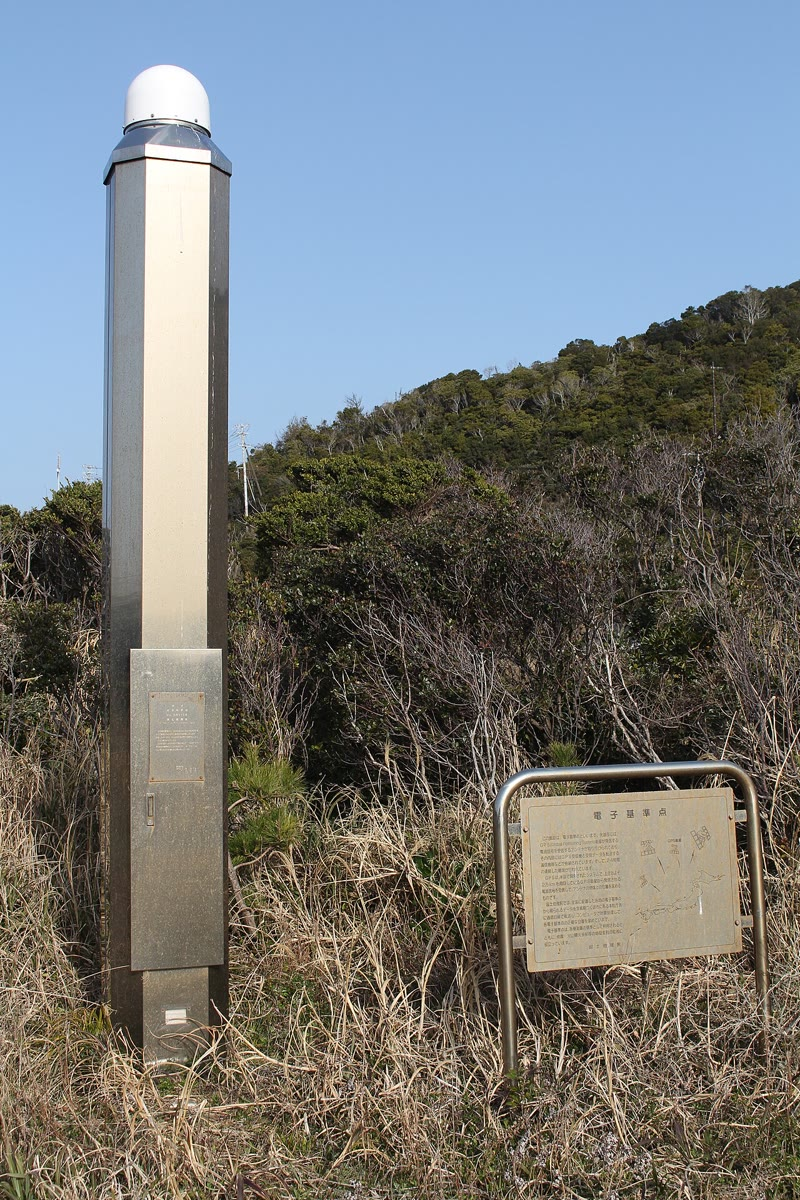
\includegraphics[width=\linewidth]{images/book3/b1-gnss-station.jpg}

{\scriptsize 日本的一个永久站，其天线位于防风雨罩之下
（Alpsdake, CC BY-SA 4.0）。}
\end{minipage}
\end{inthefield}

位于两个板块内部的台站，其速度给出一个属于它们自身的\omterm{def:b1:plate-kinematics:euler-pole}{欧拉矢量}，
且不依赖于地质记录。对于欧亚板块相对于北美板块，该矢量预测冰岛处的速率为
\qty{17.0}{mm.\text{年}^{-1}}，比在 \qty{3.16}{Ma} 内平均得到的
\qty{18.6}{mm.\text{年}^{-1}} 约小 \qty{8}{\percent}（见上图）。雷克雅未克与斯塔万格之间的弦，
两地都位于各自板块的\omterm{def:b1:plate-kinematics:triple-junction}{稳定}部分，
其长度以 \qty{17.5}{mm.\text{年}^{-1}} 的速率增长；卫星矢量预测为 \qty{17.1}{mm.\text{年}^{-1}}，
地质矢量则为 \qty{18.6}{mm.\text{年}^{-1}}。
因此，在北大西洋两侧，几十年内测得的速率
与在 300 万年内平均得到的速率相差不到十分之一：
在此处，板块今天的运动几乎与其
数百万年来的运动一致。
% ledger: morvel:gps-eu-na, morvel:eu-na, ngl:reyk, ngl:stas (chord rates computed in calc/ch12.py)

在板块边界带内，情况没有那么简单，
因为台站的运动不止来自板块。冰岛十分之一以上的面积位于冰帽之下，
其中大部分自约 1890 年起一直在失去质量：
随着荷载减小，其下的\omterm{def:b1:layered-earth:layers}{地壳}隆升，并从正在变薄的冰层处水平地向外移动。
位于东南海岸、靠近最大冰帽的霍芬站，
以 \qty{12.9}{mm.\text{年}^{-1}} 的速率隆升。
% ledger: spaans:iceland-gia, ngl:hofn

\section{练习}

全文取 $R = \qty{6371}{km}$。

\begin{exercise}[$\star$]\label{exo:b1:plate-kinematics:1}
欧亚板块相对于北美板块的\omterm{def:b1:plate-kinematics:euler-pole}{欧拉矢量}，其转动速率为
\qty{0.210}{\degree\per\Ma}。(a) 将其换算为 \unit{rad.\text{年}^{-1}} 和
\unit{rad.s^{-1}}。(b) 一整圈需要多长时间？(c) 计算 $\omega R$，单位为
\unit{mm.\text{年}^{-1}}。
% ledger: morvel:eu-na
\end{exercise}

\begin{exercise}[$\star$]\label{exo:b1:plate-kinematics:2}
使用同一\omterm{def:b1:plate-kinematics:euler-pole}{欧拉矢量}，计算两板块在距\omterm{def:b1:plate-kinematics:euler-pole}{欧拉极}
\ang{30}、\ang{60} 和 \ang{90} 处的相对速度。
沿板块边界，何处的扩张最快？
\end{exercise}

\begin{exercise}[$\star$]\label{exo:b1:plate-kinematics:3}
Jaramillo 正常亚\omterm{def:b1:plate-kinematics:magnetic-anomaly}{极性时}持续了从 \qty{1.072}{Ma} 到 \qty{0.988}{Ma}。
(a) 在\omterm{def:b1:plate-kinematics:spreading-rate}{半扩张速率}为
\qty{50}{mm.\text{年}^{-1}} 的洋脊每一侧，该亚\omterm{def:b1:plate-kinematics:magnetic-anomaly}{极性时}形成的条带宽度为多少？若为 \qty{10}{mm.\text{年}^{-1}} 呢？(b) 现今正常\omterm{def:b1:plate-kinematics:magnetic-anomaly}{极性时}
形成的条带总宽度是多少？该正常\omterm{def:b1:plate-kinematics:magnetic-anomaly}{极性时}始于
\qty{0.781}{Ma}，洋脊的半速率为 \qty{10}{mm.\text{年}^{-1}}？
% ledger: iodp:gpts2004
\end{exercise}

\begin{exercise}[$\star$]\label{exo:b1:plate-kinematics:4}
在穿过洋脊的剖面上，C2An \omterm{def:b1:plate-kinematics:magnetic-anomaly}{极性时}异常的年轻边缘，
年龄为 \qty{2.581}{Ma}，位于轴线以西 \qty{66}{km}、以东 \qty{64}{km} 处。
计算两个\omterm{def:b1:plate-kinematics:spreading-rate}{半扩张速率}和\omterm{def:b1:plate-kinematics:spreading-rate}{全扩张速率}。
扩张是否对称？
% ledger: iodp:gpts2004
\end{exercise}

\begin{exercise}[$\star\star$]\label{exo:b1:plate-kinematics:5}
北冰洋中加克尔洋脊上的一点，位于北纬 \ang{85}、东经 \ang{0}。
计算该点距欧亚–北美\omterm{def:b1:plate-kinematics:euler-pole}{欧拉极}的角距离，
（北纬 \ang{61.8}、东经 \ang{139.6}，\qty{0.210}{\degree\per\Ma}），以及该处的扩张速率。
并与实测速率 \qtyrange{11}{12}{mm.\text{年}^{-1}} 进行比较。
% ledger: morvel:eu-na
\end{exercise}

\begin{exercise}[$\star\star$]\label{exo:b1:plate-kinematics:6}
亚速尔\omterm{def:b1:plate-kinematics:triple-junction}{三联点}位于北纬 \ang{39.44}、西经 \ang{29.83}，计算 (a) 该点
距欧亚–北美\omterm{def:b1:plate-kinematics:euler-pole}{欧拉极}的角距离，(b) 扩张速率，
以及 (c) 相对运动的\omterm{def:b1:spherical-astronomy:horizontal}{方位角}。(d) 对于\omterm{def:b1:plate-kinematics:triple-junction}{三联点}以北洋脊上的转换断层，
你预测其\omterm{def:b1:field-lab-methods-1:trend-plunge}{倾伏向}如何？
% ledger: morvel:eu-na, morvel:azores
\end{exercise}

\begin{exercise}[$\star\star$]\label{exo:b1:plate-kinematics:7}
(a) 写出\omterm{def:b1:plate-kinematics:euler-pole}{欧拉矢量} $\vec\omega_{\mathrm{EU\,NA}}$
（北纬 \ang{61.8}、东经 \ang{139.6}，\qty{0.210}{\degree\per\Ma}）和 $\vec\omega_{\mathrm{NB\,NA}}$
（北纬 \ang{79.2}、东经 \ang{40.2}，\qty{0.233}{\degree\per\Ma}），
以直角坐标分量表示，单位为 \unit{\degree\per\Ma}。(b) 推导 $\vec\omega_{\mathrm{NB\,EU}}$，
给出其极点和速率。(c) 为什么这是了解努比亚板块
相对于欧亚板块运动的最佳方法？
% ledger: morvel:eu-na, morvel:nb-na
\end{exercise}

\begin{exercise}[$\star\star$]\label{exo:b1:plate-kinematics:8}
设 $\vec e_x$ 指向北纬 \ang{0}、东经 \ang{0}，$\vec e_y$ 指向北纬 \ang{0}，
东经 \ang{90}，$\vec e_z$ 指向北极。用罗德里格斯公式计算 $\vec e_x$ 的像：
(a) 先绕 $\vec e_z$ 转动 \ang{90}，
再绕 $\vec e_x$ 转动 \ang{90}；(b) 以相反顺序
进行同样的两次转动。(c) 这对板块过去
位置的重建意味着什么？
\end{exercise}

\begin{exercise}[$\star\star$]\label{exo:b1:plate-kinematics:9}
三块板块 A、B 和 C 相交于一个脊–脊–脊型\omterm{def:b1:plate-kinematics:triple-junction}{三联点}。相对于 A，
板块 B 以 \qty{30}{mm.\text{年}^{-1}} 的速率向东运动，板块 C 以
\qty{40}{mm.\text{年}^{-1}} 的速率向南运动。（a）画出速度三角形。
（b）求 C 相对于 B 的速率和\omterm{def:b1:spherical-astronomy:horizontal}{方位角}。（c）若 B 与 C 之间的洋脊
沿垂直于其轴线的方向扩张，则其\omterm{def:b1:field-lab-methods-1:trend-plunge}{倾伏向}是什么？
\end{exercise}

\begin{exercise}[$\star\star\star$]\label{exo:b1:plate-kinematics:10}
（a）证明旋转矩阵 $R$（绕任一轴转动 $\alpha$ 角）的
迹为 $1 + 2\cos\alpha$。（b）矩阵
\[
  R = \begin{pmatrix} 0 & 0 & 1\\ 1 & 0 & 0\\ 0 & 1 & 0\end{pmatrix}
\]
该矩阵正交，行列式为 $1$。求其转轴（以\omterm{def:b1:spherical-astronomy:geographic}{纬度}和\omterm{def:b1:spherical-astronomy:geographic}{经度}表示），
及其转角。（c）通过将 $R$ 作用于 $\vec e_x$、$\vec e_y$
和 $\vec e_z$ 检验你的答案。
\end{exercise}

\begin{exercise}[$\star\star\star$]\label{exo:b1:plate-kinematics:11}
卫星定位出现之前，\omterm{def:b1:plate-kinematics:euler-pole}{欧拉极}由转换断层的
\omterm{def:b1:field-lab-methods-1:trend-plunge}{倾伏向}推得。（a）证明\omterm{def:b1:plate-kinematics:euler-pole}{欧拉极}位于过转换断层某点的\omterm{def:b1:spherical-astronomy:spherical-triangle}{大圆}上，
该\omterm{def:b1:spherical-astronomy:spherical-triangle}{大圆}在该点与断层垂直，且
\omterm{def:b1:plate-kinematics:euler-pole}{欧拉极}因此沿 $\vec t_1\times\vec t_2$ 方向，其中 $\vec t_1$ 与
$\vec t_2$ 为同一边界上两条转换断层方向上的单位矢量。
（b）亚速尔\omterm{def:b1:plate-kinematics:triple-junction}{三联点}附近转换断层的\omterm{def:b1:field-lab-methods-1:trend-plunge}{倾伏向}为 \ang{95}
（北纬 \ang{39.44}，西经 \ang{29.83}），冰岛附近为 \ang{103}（北纬 \ang{64.5}，
西经 \ang{18}）。在\omterm{def:b1:spherical-astronomy:geographic}{纬度} $\varphi$、\omterm{def:b1:spherical-astronomy:geographic}{经度}
$\lambda$ 处指向\omterm{def:b1:spherical-astronomy:horizontal}{方位角} $\beta$ 的水平单位矢量为 $\sin\beta\,\vec e +
\cos\beta\,\vec n$，其中 $\vec e = (-\sin\lambda, \cos\lambda, 0)$ 且 $\vec n =
(-\sin\varphi\cos\lambda, -\sin\varphi\sin\lambda, \cos\varphi)$。求
\omterm{def:b1:plate-kinematics:euler-pole}{欧拉极}的位置。（c）两条转换断层能在多大程度上确定\omterm{def:b1:plate-kinematics:euler-pole}{欧拉极}？
% ledger: morvel:eu-na
\end{exercise}

\begin{exercise}[$\star\star\star$]\label{exo:b1:plate-kinematics:12}
某台站每三个月测得一次、持续三年的东向位置
（以毫米计，自 $t = 0$ 起）如下：
\begin{center}\small
\begin{tabular}{l*{13}{c}}
\hline
$t$（年） & 0 & 0.25 & 0.5 & 0.75 & 1 & 1.25 & 1.5 & 1.75 & 2 & 2.25 & 2.5 & 2.75 & 3\\
$x$（毫米） & 4 & 5 & 6 & 15 & 24 & 25 & 26 & 65 & 74 & 75 & 76 & 85 & 94\\
\hline
\end{tabular}
\end{center}
该序列由\omterm{def:b1:plate-kinematics:triple-junction}{稳定}运动、季节性振荡以及一次
由地震引起的跳变组成。（a）由首末两个位置求速度。
（b）计算相隔恰好一年的两位置之差（共九个）及其
中位数。（c）解释为何一年间隔差值的中位数是一个稳健的
\omterm{def:b1:plate-kinematics:triple-junction}{稳定}速度估计，以及在何种情况下它会失效。
\end{exercise}

\section{问题：冰岛裂开}

\begin{problem}[{周末问题——北大西洋穿越冰岛的张开，
以三种方式测量}]
\label{pb:b1:plate-kinematics:1}
% values: calc/ch12.py (Part II profile invented for the problem; real Euler
% vectors, chron ages and station velocities)
% ledger: morvel:eu-na, morvel:nb-na, iodp:gpts2004, ngl:reyk, ngl:stas, ngl:hofn
冰岛位于大西洋中脊上，夹在西侧的北美板块与
东侧的欧亚板块之间。取 $R = \qty{6371}{km}$，并对
欧亚板块相对于北美板块，取\omterm{def:b1:plate-kinematics:euler-pole}{欧拉矢量}，其\omterm{def:b1:plate-kinematics:euler-pole}{欧拉极}位于
北纬 \ang{61.8}，东经 \ang{139.6}，角速率为 \qty{0.210}{\degree\per\Ma}。

\medskip
\noindent\textbf{第一部分——板块矢量。}
\begin{enumerate}
  \item 将速率换算为 \unit{rad.\text{年}^{-1}}，并计算 $\omega R$
        （以 \unit{mm.\text{年}^{-1}} 为单位）。
  \item 计算从极点到冰岛中心的角距离 $\Delta$，
        （北纬 \ang{64.5}，西经 \ang{18}）。
  \item 推出板块矢量所预测的穿过冰岛的
        \omterm{def:b1:plate-kinematics:spreading-rate}{全扩张速率}。
  \item 计算从冰岛看去极点的\omterm{def:b1:spherical-astronomy:horizontal}{方位角}，以及
        欧亚板块相对于北美板块运动的\omterm{def:b1:spherical-astronomy:horizontal}{方位角}。
  \item 将该速度分解为向东和向北的分量。
  \item 在加克尔洋脊（北纬 \ang{86}，东经 \ang{60}）处，相同矢量给出的
        速率是多少？该处边界为何慢得多？
\end{enumerate}

\noindent\textbf{第二部分——磁条带。}
一艘船沿雷克雅内斯洋脊（位于冰岛西南，靠近
北纬 \ang{63}，西经 \ang{23}）沿扩张方向航行，测得的磁剖面给出
从洋脊轴线到三个\omterm{def:b1:plate-kinematics:magnetic-anomaly}{极性时}边界的距离
（为本题构造的剖面）：
\begin{center}\small
\begin{tabular}{lccc}
\hline
边界 & 年龄（Ma） & 轴线以西（千米） & 轴线以东（千米）\\
\hline
C1n 底界 & 0.781 & 9.7 & 10.1\\
C2An 的年轻边界 & 2.581 & 26.8 & 27.3\\
C5n 的年轻边界 & 9.779 & 94 & 97\\
\hline
\end{tabular}
\end{center}
\begin{enumerate}[resume]
  \item 由 C5n 的年轻边界，计算两个\omterm{def:b1:plate-kinematics:spreading-rate}{半扩张速率}。
  \item 推出自 \qty{9.8}{Ma} 以来的\omterm{def:b1:plate-kinematics:spreading-rate}{全扩张速率}。
  \item 同样由两个较年轻的边界计算\omterm{def:b1:plate-kinematics:spreading-rate}{全扩张速率}，三者
        是否一致？请描述它们如何随边界年龄而变化。
  \item 扩张是否对称？这种不对称是否会改变\omterm{def:b1:plate-kinematics:spreading-rate}{全扩张速率}？
  \item 在雷克雅内斯洋脊上，各条带之间的边界
        相对轴线向外错移，两侧合计 \qty{5.0}{km}。
        校正三个\omterm{def:b1:plate-kinematics:spreading-rate}{全扩张速率}。为何该校正对最年轻
        的边界影响最大？
  \item 求 Jaramillo 亚\omterm{def:b1:plate-kinematics:magnetic-anomaly}{极性时}的条带
        （\qtyrange{1.072}{0.988}{Ma}）在每一侧的宽度，按校正后的\omterm{def:b1:plate-kinematics:spreading-rate}{半
        扩张速率}计算？将其与第 11 题的位移相比较。Jaramillo
        异常仍能在雷克雅内斯洋脊剖面上清楚识别，
        但在加克尔洋脊上缺失：这说明什么？
  \item 板块矢量在该剖面处预测速率为 \qty{19.0}{mm.\text{年}^{-1}}。
        将其与你校正后的各速率比较。
\end{enumerate}

\noindent\textbf{第三部分——卫星。}
常驻站 REYK（雷克雅未克，北纬 \ang{64.139}，西经 \ang{21.955}）与
STAS（斯塔万格，北纬 \ang{59.018}，东经 \ang{5.599}）分别位于北美板块和
欧亚板块上。其实测速度使两站间的弦长
每年增长 \qty{17.5}{mm.\text{年}^{-1}}。
\begin{enumerate}[resume]
  \item 求两站间的角距离，以及
        弦长。
  \item 弦长增长一米需要多长时间？
  \item 板块矢量给出 STAS 的速度为 \qty{18.9}{mm.\text{年}^{-1}}，相对北美
        指向 \ang{114.8}。从 REYK 出发的\omterm{def:b1:spherical-astronomy:spherical-triangle}{大圆}
        到达 STAS 时的方向为 \ang{123.1}。求速度沿此方向的分量，
        再求弦长的预测增长量，
        其中弦与 STAS 处的水平面成夹角 $\Delta/2$。
  \item 比较实测增长量与预测增长量。
        造成两者差异的原因可能是什么？
  \item 相对北美，REYK 以 \qty{1.07}{mm.\text{年}^{-1}} 向
        西、以 \qty{0.97}{mm.\text{年}^{-1}} 向南运动，台站 HOFN（霍芬，
        冰岛东南部）以 \qty{21.12}{mm.\text{年}^{-1}} 向东，
        以 \qty{6.97}{mm.\text{年}^{-1}} 向南运动。求 HOFN
        相对 REYK 的速率与\omterm{def:b1:spherical-astronomy:horizontal}{方位角}。
  \item 与第一部分比较。HOFN 也上升 \qty{12.9}{mm.\text{年}^{-1}}。为何
        位于冰岛内部的台站难以很好地度量板块运动？
\end{enumerate}

\noindent\textbf{第四部分——一千万年，以及南方的\omterm{def:b1:plate-kinematics:triple-junction}{三联点}。}
\begin{enumerate}[resume]
  \item 在 \qty{10}{Ma} 的时间内，欧亚板块相对
        北美绕该极点转过多大角度？
  \item 位于冰岛中部的欧亚板块上一点，沿其\omterm{def:b1:spherical-astronomy:spherical-triangle}{小圆}
        在该时间内行进多远？请与第二部分中
        自 C5n 年轻边缘以来形成的\omterm{def:b1:layered-earth:layers}{地壳}校正宽度作比较。
  \item 在亚速尔\omterm{def:b1:plate-kinematics:triple-junction}{三联点}处，板块矢量给出欧亚板块的速度为
        \qty{22.9}{mm.\text{年}^{-1}}，指向 \ang{95.1}；努比亚板块为
        \qty{19.2}{mm.\text{年}^{-1}}，指向 \ang{103.8}（均相对北美）。
        求欧亚板块相对努比亚板块的速度。
  \item 该\omterm{def:b1:plate-kinematics:triple-junction}{三联点}是否\omterm{def:b1:plate-kinematics:triple-junction}{稳定}？
        由第 22 题的速度可知，欧亚板块与努比亚板块之间是何种边界？
  \item 汇总第一、第二和第三部分的扩张速率。哪些结果相互一致，
        以及哪种方法在最短时间内度量板块运动？
  \item 精确到每年毫米，板块矢量与校正后的磁条带
        各给出穿越冰岛的\omterm{def:b1:plate-kinematics:spreading-rate}{全扩张速率}。两者分别为
        多少？
\end{enumerate}
\end{problem}
